%%%%%%%%%%%%%%%%%%%%%%%%%%%%%%%%%%%%%%%%%%%%%%%%%%%%%%%%%%%%%%%%%%%%%%
% How to use writeLaTeX: 
%
% You edit the source code here on the left, and the preview on the
% right shows you the result within a few seconds.
%
% Bookmark this page and share the URL with your co-authors. They can
% edit at the same time!
%
% You can upload figures, bibliographies, custom classes and
% styles using the files menu.
%
%%%%%%%%%%%%%%%%%%%%%%%%%%%%%%%%%%%%%%%%%%%%%%%%%%%%%%%%%%%%%%%%%%%%%%

\documentclass[12pt]{article}

\usepackage{sbc-template}

\usepackage{graphicx,url}
\usepackage[section]{placeins}

\usepackage[brazil]{babel}   
\usepackage[utf8]{inputenc}  
\usepackage{amsmath}
\usepackage{amsfonts}
\usepackage[shortlabels]{enumitem}
\usepackage{cleveref}

\graphicspath{ {./images/} }

%Inclui () nas citações
\usepackage{cite}
\renewcommand\citeleft{(}
\renewcommand\citeright{)}
\renewcommand{\email}[1]{\\\mbox{}\\[-6pt]\footnotesize\ttfamily\begin{tabular}{@{} c @{}}#1\end{tabular}}





     
\sloppy

\title{Caixeiro viajante com deadline aplicado\\ para a minimização de atraso de chegada em N localidades}

\author{Breno C. Zukowski\inst{1}, Henrique Ribeiro dos Santos\inst{1}, Jean Luca dos Santos Silva\inst{1}, \\ Paola Paulina D. J. S. Capita\inst{1}}


\address{Faculdade de Tecnologia de Ribeirão Preto - (FATEC)\\
  Ribeirão Preto, SP -- Brasil
  \email{breno.marques@fatec.sp.gov.br, henrique.santos54@fatec.sp.gov.br, \\ jean.silva88@fatec.sp.gov.br,paola.capita@fatec.sp.gov.br}}

\begin{document}

\maketitle
\begin{abstract}
  The traveling salesman problem is a classic of mathematical literature, where a salesperson must visit a set of N cities once and return to his point of origin, through a route that minimizes the traveled distance. This work proposes a solution with a mathematical programming model, for a variant of the original problem that has time limits for arrival at each city, in which delays are allowed and the objective is to minimize the overall delay of the route. Using the PyMathProg library we achieved interesting results, offering plausible routes to the points offered.\end{abstract}

\begin{resumo}
  O problema do caixeiro viajante é um clássico da literatura matemática, onde um vendedor deve visitar um conjunto de N cidades uma única vez e retornar ao seu ponto de origem, através de uma rota que minimiza a distância percorrida. Este trabalho propõe uma solução via modelo de programação matemática, para uma variante do problema original que conta com tempos limite para chegada a cada cidade, em que atrasos são permitidos e têm-se como objetivo minimizar o atraso geral da rota. Com a utilização da biblioteca PyMathProg atingimos resultados interessantes, oferecendo rotas plausíveis para os pontos oferecidos.
\end{resumo}


\section{Introdução}
Os problemas de roteirização e otimização de tempo são grandes conhecidos do cotidiano, não é incomum que uma rota tenha diversas possibilidades de percurso. Este tipo de problema é explorado há séculos, sendo um dos seus exemplos mais famosos o Problema do Caixeiro Viajante (PCV), problema este trabalhado desde o século XIX por diversos matemáticos. Com o advento da Pesquisa Operacional (PO), este tipo de situação começou a tomar novas proporções através da utilização de modelos matemáticos e programação de computadores para obter soluções eficientes para diversas variações do PCV.

A PO é a área do conhecimento dedicada a estudar e aplicar métodos analíticos para a resolução de problemas nas mais diversas áreas de atuação humana \cite{sobrapo2017}. A partir dela somos capazes de encontrar soluções ótimas com limitações de recursos e restrições, modelando matematicamente a realidade para obter resultados factíveis para a resolução de diversas situações \cite{hillier2013introdução}.

Neste trabalho exploramos Problema do Caixeiro Viajante com tempo limite de chegada utilizando uma abordagem desenvolvida em aula que será descrita em detalhes na próxima sessão.



\section{Descrição do problema}

O problema do caixeiro viajante é um clássico da otimização combinatória, que propõe que um determinado caixeiro deverá visitar {\it n} cidades diferentes, iniciando e encerrando sua viagem na primeira cidade. A ordem das cidades visitadas é irrelevante e de cada uma delas pode-se ir diretamente a qualquer outra \cite{porto-da-silveira_2000}. Trata-se de um problema de complexidade $R(n) = (n -1)!$ e pertence a classe dos NP-completos. Até o presente momento este é um problema aberto da matemática, sem resolução polinomial descoberta.

Tendo em vista essas informações, existem também variações do PCV e a partir de uma destas desenvolvemos o seguinte trabalho. Dado o enunciado temos:


\begin{enumerate}[(a)]
  \item Um veículo que deve partir do ponto inicial, visitará {\it n} localidades e retornará ao ponto de partida após as visitas.
  \item Cada localidade a ser visitada tem um prazo limite para receber a visita.
  \item Atrasos são permitidos, porém uma multa que aumenta com o tempo de atraso é imposta.
  \item A distância euclidiana (em linha reta) entre as localidades é contabilizada como tempo de percurso.
\end{enumerate}

O modelo deverá minimizar o atraso total das visitas, eliminando sub-rotas e garantindo que as restrições sejam devidamente atendidas.


\section{Modelagem Matemática}

\subsection{Conjunto de Nós}

Representativamente podemos definir um conjunto de valores N como visto em \eqref{nodes} para todos os nós $n$, sendo que 0 e $n+1$ representam o ponto de origem que também deverá ser o último nó a ser visitado ao fim do percurso.

\begin{align}
  N = \{0, ..., n+1\} \label{nodes}
\end{align}

Concomitantemente temos o produto cartesiano destes nós dado por:

\begin{align} \label{cartesian_product}
   & A = N * N
\end{align}

\subsection{Função Objetivo:}

A função objetivo abaixo mostra a minimização do somatório do atraso nos nós, representado pela variável $w_j$:

\begin{align}
  min        \sum_{_j\in N\backslash \{0,n+1\}} w_j \label{obj_func}
\end{align}

\subsection{Restrições:}

A restrição \eqref{res_x1} mostra o somatório entre todas as variáveis $x_{ij}$ que necessariamente terá que equivaler a 1, definindo que apenas um arco é utilizado nessa roteirização, fixando os pontos de chegada. A expressão \eqref{res_x2} tem função similar, por sua vez, restringindo os pontos de saída. Estas restrições garantem que os nós tenham pontos de chegada e partida únicos.


\begin{align}
   & \sum_{i\in N\backslash \{n+1\}} x_{ij} = 1 &  & j\in N\backslash \{0\} \label{res_x1}
\end{align}

\begin{align}
   & \sum_{j\in N\backslash \{0\}} x_{ij} = 1 &  & i\in N\backslash \{n+1\} \label{res_x2}
\end{align}

Abaixo podemos ver a restrição \eqref{sub-routes} que garante que não ocorram sub-rotas. A variável $\varphi$ representa o instante de início do serviço em um nó $i \in N$. Caso o nó $x_{ij}$ não seja utilizado, a constante $M_{ij}$ que é suficientemente grande, garante que toda a expressão assuma um valor negativo, portanto $\varphi_j$ poderá assumir qualquer valor.

\begin{align}
   & \varphi_j \geq \varphi_i + (S_i + t_{ij})x_{ij} - M_{ij}(1-x_{ij}) &  & i\in N\backslash \{n+1\} &  & j\in N\backslash \{0\} \label{sub-routes}
\end{align}

A restrição \eqref{delay} garante que o acúmulo de atraso $w_j$ seja maior que o tempo de chegada de um nó $i \in N$ subtraído da {\it deadline}. Nesta restrição não estão inclusos os nós $0$ e $n+1$ já que estes são considerados depósitos e não possuem {\it deadline}.

\begin{align}
   & w_j \geq \varphi_j - D_j & \label{delay} & j\in N\backslash \{0,n+1\}
\end{align}

A restrição \eqref{res_wj} abaixo garante e não-negatividade de $w_j$
\begin{align}
   & w_j \geq 0 &  & j\in N\backslash \{0,n+1\} \label{res_wj}
\end{align}

Por fim, a restrição \eqref{variables} declara o domínio de valores possíveis para a variável $x_{ij}$.
\begin{align}
   & x_{ij} \in \{0,1\} &  & i\in N\backslash \{n+1\} &  & j\in N\backslash \{0\}  \label{variables}
\end{align}


\subsection{Variáveis:}

\hspace{1.27cm}$w_j$ Tempo de atraso para cada nó de chegada $j$.

\hspace{1.27cm} $j\in N\backslash \{0,n+1\}$

$x_{ij}$ Variável binária que define se o arco é utilizado na rota.

\hspace{1.27cm} $i\in N\backslash \{n+1\}$ \hspace{1.27cm}  $j\in N\backslash \{0,n+1\}$

$\varphi$ Variável de decisão contínua que representa o instante de inicio do serviço de um nó $i\in N$.

\hspace{1.27cm} $(i,j) \in A$

$D_j$ {\it Deadline} de chegada para um nó $j$.

\hspace{1.27cm} $j\in N\backslash \{0,n+1\}$

$t_{ij}$ Distância euclidiana entre um nó e outro.

\hspace{1.27cm} $i\in N\backslash \{n+1\}$ \hspace{1.27cm}  $j\in N\backslash \{0,n+1\}$

$S_i$ Tempo de serviço em um nó.

\hspace{1.27cm} $i\in N\backslash \{n+1\}$

$M$ Valor suficientemente grande.


\section{Resultados Computacionais}
O modelo \eqref{obj_func}-\eqref{variables} foi codificado na linguagem de programação Python em conjunto com a biblioteca PyMathProg, que possibilita a elaboração e solução de problemas de programação matemática, e com a biblioteca MatplotLib que permite a criação de visualizações estáticas, animadas e interativas.(https://matplotlib.org/)
A biblioteca PyMathProg faz uso do solver GLPK (GNU Linear Programming Kit) que tem a função de resolver problemas de programação linear em larga escala (LP), programação inteira mista (MIP) e outros problemas relacionados. (https://www.gnu.org/software/glpk/).

Para realizar os testes com o modelo matemático elaborado, utilizamos 4 instâncias com dados fictícios, incluindo as coordenadas (x e y), o tempo de serviço e o deadline (tempo máximo de chegada) para cada nó.
Cada instância tem, respectivamente, 10, 15, 20 e 25 nós. A partir da instância com 15 nós, o tempo de execução dos modelos foi limitado a 2 horas.
O ambiente de execução possui as seguintes características:

% Não sei se fica melhor como lista ou tabela e se fica melhor aqui ou no final
\begin{enumerate}[-]
  \item Processador: Intel i7-10510U (8) 4.900GHz
  \item Placa de video: NVIDIA GeForce MX230
  \item Memória RAM: 16gb DDR4
  \item Sistema operacional: Ubuntu 22.04 LTS
  \item Arquitetura: 64 bits
\end{enumerate}

% Nome da instancia, tempo decorrido, valor ótimo(tempo de atraso), gap (porcentagem), limitante inferior e superior

\begin{table}[h!]
  \begin{center}
    \caption{Resultados computacionais.}
    \label{tab:table1}
    \begin{tabular}{l|c|c|c|c|c} % <-- Alignments: 1st column left, 2nd middle and 3rd right, with vertical lines in between
      \textbf{Instância} & \textbf{Tempo decorrido} & \textbf{Valor ótimo} & \textbf{Gap} & \textbf{Lim. inferior} & \textbf{Lim. superior} \\
      \hline
      inst\_10           & 3.12                     & 147.76               & 0            & 1.47                   & 1.47                   \\
      \hline
      inst\_15           & 7200.10                  & 77.28                & 100          & 7.72                   & 0                      \\
      \hline
      inst\_20           & 7200.15                  & 329.76               & 100          & 3.29                   & 0                      \\
      \hline
      inst\_25           & 7200.27                  & 1124.18              & 100          & 1.12                   & 0                      \\
      \hline
    \end{tabular}
  \end{center}
\end{table}



Abaixo seguem as representações do percurso encontrado para cada instância, onde o ponto vermelho indica o nó de partida e chegada. As rotas que se cruzam não são um problema, já que o objetivo é minimizar o atraso e não o percurso.
\linebreak
Na primeira instância o programa conseguiu encontrar uma solução ótima em pouco mais que 3 segundos, diferente das outras instâncias em que a quantidade de nós aumentou significativamente a complexidade do problema. Podemos ver as rotas plotadas na figura 1.

% Aqui teve solução ótima, nas outras foram soluções aproximadas.
% pra editar as figuras segui essa doc: 
% https://pt.overleaf.com/learn/latex/Inserting_Images
\begin{figure}[ht]
  \centering
  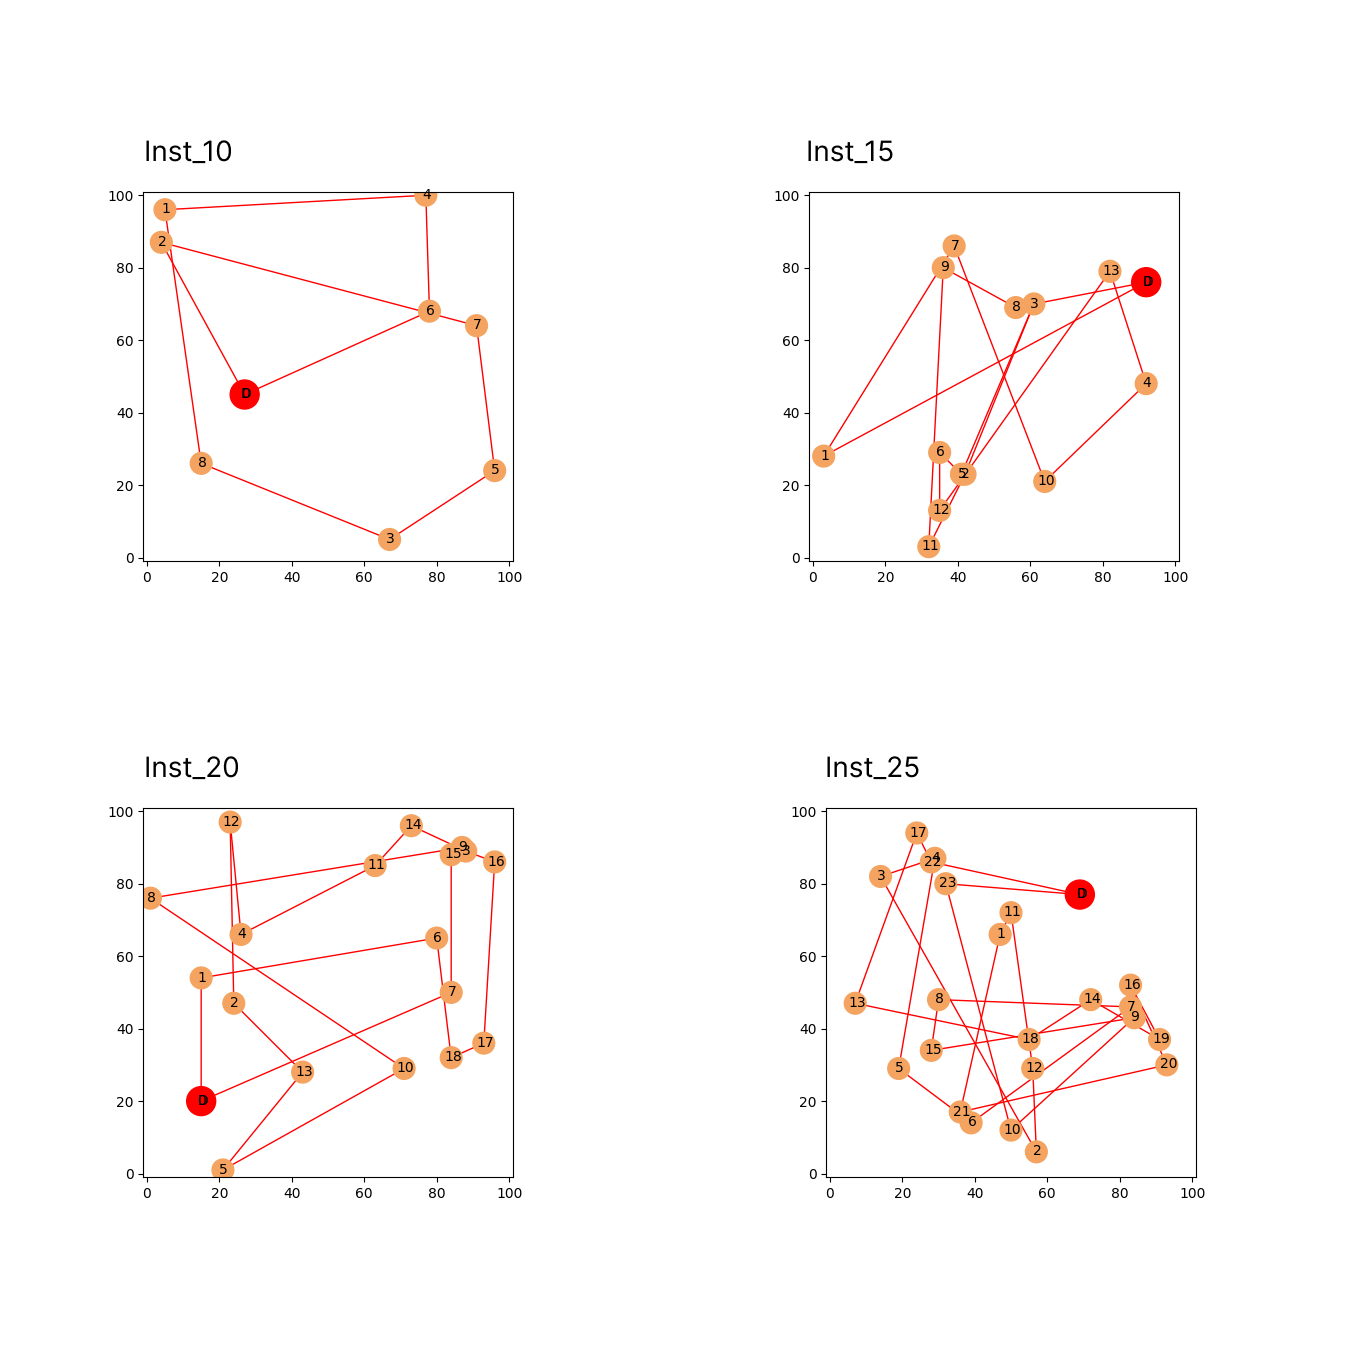
\includegraphics[scale=0.3]{imagens/images_compiled.png}
  \label{graph_inst}
  \caption{Aqui podemos ver respectivamente todas as rotas plotadas durante a análise das instâncias. Em ordem temos os conjuntos de dados seguintes: inst\_10, inst\_15, inst\_20 e inst\_25.}

\end{figure}

\FloatBarrier

\section{Considerações Finais}

Lorem ipsum solor dolor armet etc askopsakopaskopaskopsadkopasdkopaskdopaksdopkasd



\bibliographystyle{abnt}
\bibliography{sbc-template}

\end{document}